% -*- compile-command: "make HOCKING-slides.pdf" -*-
\documentclass{beamer}
\usepackage{tikz}
\usepackage[all]{xy}
\usepackage{amsmath,amssymb}
\usepackage{hyperref}
\usepackage{graphicx}
\usepackage{algorithmic}
\usepackage{multirow}

%\usepackage{appendixnumberbeamer}

\addtobeamertemplate{navigation symbols}{}{%
    \usebeamerfont{footline}%
    \usebeamercolor[fg]{footline}%
    \hspace{1em}%
    \insertframenumber/\inserttotalframenumber
}

\DeclareMathOperator*{\argmin}{arg\,min}
\DeclareMathOperator*{\Lik}{Lik}
\DeclareMathOperator*{\Peaks}{Peaks}
\DeclareMathOperator*{\Segments}{Segments}
\DeclareMathOperator*{\argmax}{arg\,max}
\DeclareMathOperator*{\maximize}{maximize}
\DeclareMathOperator*{\minimize}{minimize}
\newcommand{\sign}{\operatorname{sign}}
\newcommand{\RR}{\mathbb R}
\newcommand{\ZZ}{\mathbb Z}
\newcommand{\NN}{\mathbb N}
\definecolor{pDPA}{HTML}{1B9E77}
\definecolor{PELT}{HTML}{D95F02}
\definecolor{FPOP}{HTML}{7570B3}
\newcommand{\algo}[1]{\textcolor{#1}{#1}}
\definecolor{PDPA}{HTML}{66C2A5}
\definecolor{CDPA}{HTML}{FC8D62}
\definecolor{GPDPA}{HTML}{4D4D4D}




% Set transparency of non-highlighted sections in the table of
% contents slide.
\setbeamertemplate{section in toc shaded}[default][100]
\AtBeginSection[]
{
  \setbeamercolor{section in toc}{fg=red} 
  \setbeamercolor{section in toc shaded}{fg=black} 
  \begin{frame}
    \tableofcontents[currentsection]
  \end{frame}
}

\begin{document}

\title{Applications of machine learning}
  \date{15 January 2019}
\author{
  Toby Dylan Hocking\\
  toby.hocking@nau.edu
}

\maketitle

% \begin{frame}
%   \frametitle{Toby Dylan Hocking, brief CV}
%   \begin{description}
%   \item[2002-2006] UC Berkeley, double major in Molecular Cell Biology
%     and Statistics (honors thesis with Terry Speed).
%   \item[2006-2008] Biochemistry (DNA-binding specificity of zinc
%     finger proteins) and statistics at Sangamo BioSciences.
%   \item[2008-2009] Masters in Statistics, Paris 6.
%   \item[2009-2012] PhD in Mathematics from Ecole Normale Superieure de
%     Cachan, machine learning for cancer genomics with JP Vert (Inst Curie)
%     and Francis Bach (INRIA).
%   \item[2013] Postdoc in Computer Science (machine learning) with Masashi Sugiyama at Tokyo
%     Institute of Technology.
%   \item[2014-2017] Postdoc on machine learning for epigenomics
%     at McGill with Guillaume Bourque.
%   \end{description}
% \end{frame}

% \section{Introduction to machine learning}

\begin{frame}
  \frametitle{Machine learning intro: image classification example}
  ML is all about learning predictive functions $f(x)\approx y$, where 
  \begin{itemize}
  \item Inputs/features $x$ can be easily computed using traditional
    algorithms, e.g. matrix of pixel intensities in an image.
  \item Outputs/labels $y$ are what we want to predict, easy to get by
    asking a human, but hard to compute using traditional algorithms,
    e.g. image class.
  \item Input $x$ = image of digit, output $y\in\{0,1,\dots,9\}$, \\--
    this is a classification problem with 10 classes.\\
  $f(
\includegraphics[height=1cm]{mnist-0})=0$,
  $f(
\includegraphics[height=1cm]{mnist-1})=1$
\item Traditional/unsupervised algorithm: I give you a pixel intensity matrix
  $x\in\RR^{16\times 16}$, you code a function $f$ that returns one of
  the 10 possible digits. Q: how to do that?
  \end{itemize}
\end{frame}

\begin{frame}
  \frametitle{Supervised machine learning algorithms}

  I give you a training data set with paired inputs/outputs, e.g.

  \begin{center}
    \Huge 0 1 2 3 4 5 6 7 8 9

  \includegraphics[height=1.9in]{mnist-digits}
  \end{center}

  Your job is to code an algorithm that learns the function $f$ from
  the training data. (you don't code $f$)
  
  \scriptsize Source: github.com/cazala/mnist
\end{frame}

\begin{frame}
  \frametitle{Advantages of supervised machine learning}

  \begin{center}
      \begin{tabular}{cc}
        \includegraphics[height=1.5in]{mnist-digits} &
  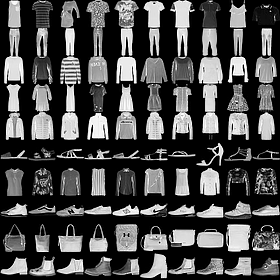
\includegraphics[height=1.5in]{fashion-mnist-sprite-some}  
  \end{tabular}
  \end{center}
  \vskip -0.2cm
  
  \begin{itemize}
  \item Input $x\in\RR^{16\times 16}$, output $y\in\{0,1,\dots,9\}$ types the same!
  \item Can use same learning algorithm regardless of pattern.
  \item Pattern encoded in the labels (not the algorithm).
  \item Useful if there are many un-labeled data, but few labeled data
    (or getting labels is long/costly).
  \item State-of-the-art accuracy (if there is enough training data).
  \end{itemize}

  \scriptsize Sources: github.com/cazala/mnist, github.com/zalandoresearch/fashion-mnist

\end{frame}

\begin{frame}
  \frametitle{Learning two different functions}
  Say \textsc{Learn} is a learning algorithm you have coded.
  \begin{center}
      \begin{tabular}{c}
        \textsc{Learn}(\includegraphics[height=1in]{mnist-digits}) $\rightarrow f$, 
        \textsc{Learn}(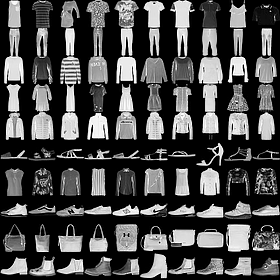
\includegraphics[height=1in]{fashion-mnist-sprite-some}) $\rightarrow g$
  \end{tabular}
  \end{center}
  \begin{itemize}
  \item Then we would expect
    $f(
\includegraphics[height=1cm]{mnist-0})=0$,
    $f(
\includegraphics[height=1cm]{mnist-1})=1$
  \item $g(
\includegraphics[height=1cm]{fashion-mnist-boot})=\text{shoe/0}$,
  $g(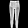
\includegraphics[height=1cm]{fashion-mnist-pants})=\text{pants/1}$
  \item Q: what happens if you do 
    $f(
\includegraphics[height=1cm]{fashion-mnist-boot})$, or
   $g(
\includegraphics[height=1cm]{mnist-0})$?

  \end{itemize}
\end{frame}

\begin{frame}
  \frametitle{Machine learning for cell image classification}
  Jones {\it et al.} PNAS 2009. Scoring diverse cellular morphologies in
  image-based screens with iterative feedback and machine learning.

\parbox{2in}{
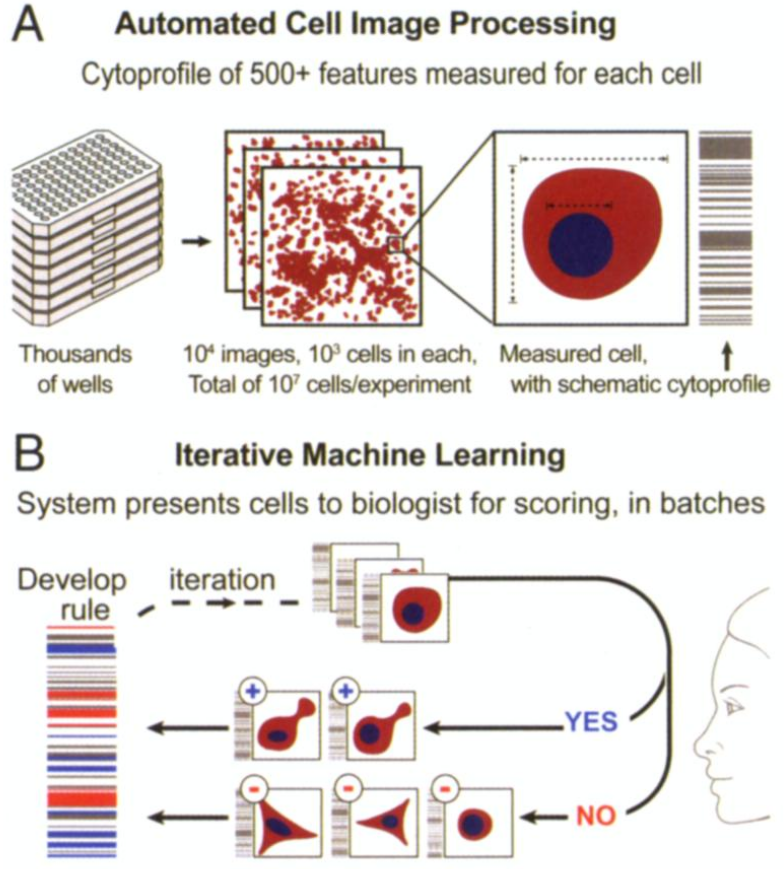
\includegraphics[width=2in]{cellprofiler} 
}
\parbox{2in}{
\begin{itemize}
  \item Input $x$ = image of cell, 
  \item Output $y\in\{\text{yes}, \text{no}\}$ (binary classification),
  \item $f(
\includegraphics[height=1cm]{cellprofiler-yes})=\text{yes}$,
  \item $f(
\includegraphics[height=1cm]{cellprofiler-no})=\text{no}$.
  \end{itemize}
}
\end{frame}


\begin{frame}
  \frametitle{Advantages of supervised machine learning}

  \begin{itemize}
  \item Can use same learning algorithm regardless of pattern.
  \item Pattern encoded in the labels (not the algorithm).
  \item State-of-the-art accuracy (if there is enough training data).
  \end{itemize}

  \begin{center}
      \begin{tabular}{cc}
        \includegraphics[height=1in]{mnist-digits} &
  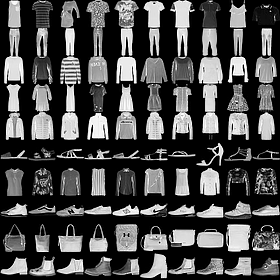
\includegraphics[height=1in]{fashion-mnist-sprite-some}  
  \end{tabular}
  \end{center}
  
  \vskip -0.2cm
  \scriptsize Sources: github.com/cazala/mnist, github.com/zalandoresearch/fashion-mnist

  %\includegraphics[width=\textwidth]{figure-good-bad}
\end{frame}



\end{document}

 